\chapter{Results}
\label{cha:Results}

TODO remake everything with the mixed light training
check all numbers

\section{Eval for question 1}

The trained policy was evaluated on tracks of all difficulty settings with the standard light setting using the Basic Evaluation algorithm \ref{sec:eval_model_track} with 100 episodes per setting. The success rates for the different difficulty settings are shown in figure \ref{fig:result_success_rates_standard}. Example videos of the agent's behaviour during evaluation can be found in the appendix \ref{cha:example_videos}.

\subsection{Experiment Results}

\begin{figure}
    \centering
    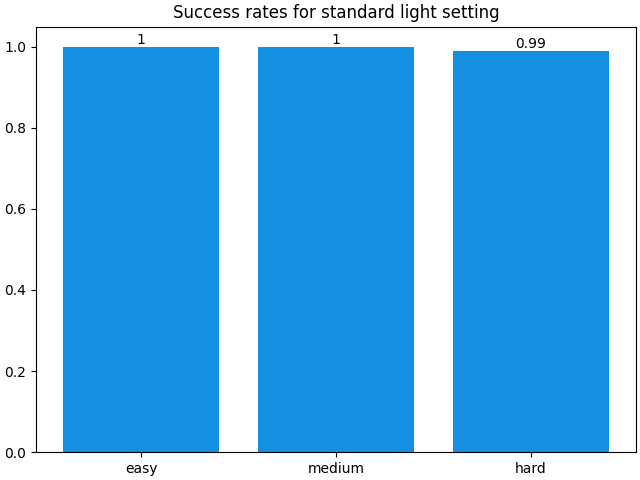
\includegraphics[width=0.45\textwidth]{Bilder/notebook_images/hardDistanceMixedLight_eval_standard_success_rates_barplot.png}
    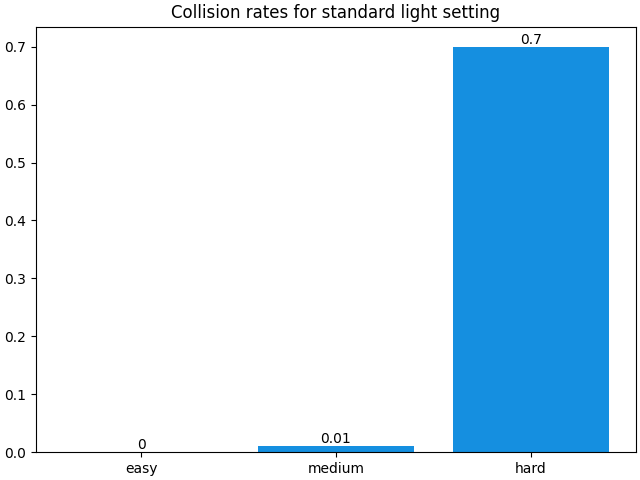
\includegraphics[width=0.45\textwidth]{Bilder/notebook_images/hardDistanceMixedLight_eval_standard_collision_rates_barplot.png}
    \caption{Success and collision rates for standard light setting.}
    \label{fig:result_success_rates_standard}
\end{figure}


The policy completed the easy, medium and hard tracks with a succes\_rate of 100\%, 93\% and 97\%. The collision\_rates were 0\%, 11\% and  29\%. The collision rates increase for the higher difficulty tracks.

\subsection{Discussion}

The trained policy is able to complete all difficulty levels very reliably.
Especially for higher difficulty settings the agent does not avoid collisions completely. The analysis of successful episodes with collisions shows that these collisions are only minor collisions. The agent collides with the goal obstacles at its side. The agent basically scapes against the goal posts.

The policy was trained on the difficult setting only. The policy did not see easy and medium difficulty parcours before the evaluation. The policy is able to generalize to tracks of lower difficulty.

TODO explain the agent behaviour (movement)
(the agent passes the goals close to the middle of the arena, not the middle of the goal)

\section{Eval for question 2}

The most succesfull model was used to evaluate the agent's performance under different light settings. The agent was evaluated on the standard, dark and bright light settings. Each combination of difficulty and light setting was evaluated with the Basic Evaluation Algorithm for 100 episodes. The success rates for the different light settings are shown in figure \ref{fig:result_success_rates_lightSettings}.


\subsection{Experiment Results}

\begin{figure}
    \centering
    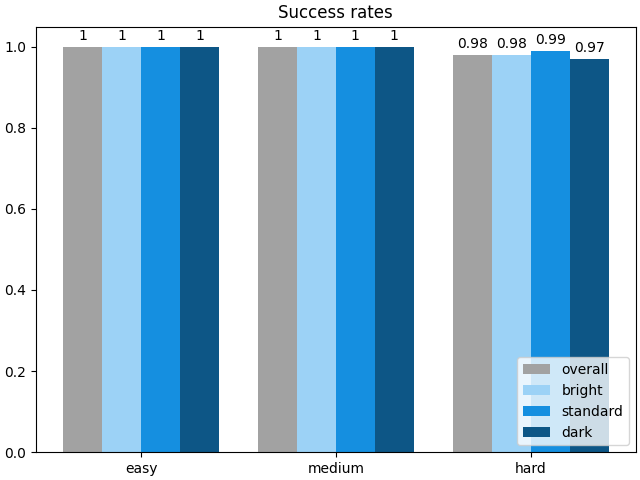
\includegraphics[width=0.45\textwidth]{Bilder/notebook_images/hardDistanceMixedLight_eval_all_success_rates_barplot.png}
    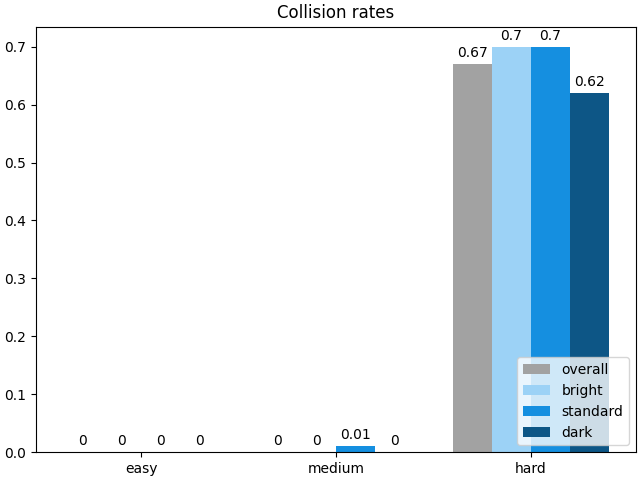
\includegraphics[width=0.45\textwidth]{Bilder/notebook_images/hardDistanceMixedLight_eval_all_collision_rates_barplot.png}
    \caption{Success and collision rate comparisons for light settings.}
    \label{fig:result_success_rates_lightSettings}
\end{figure}

The success rates for all light and difficulty settings are very high. The evaluations for the bright and dark light settings show slight differences in performance compared to the standard light setting for medium and hard tracks. The light setting had no influence on the success\_rate for the easy tracks. The agent completed the easy tracks for all light settings with a success rate of 100\%.
Most notably the success rate for medium tracks even increased by 3\% percent for the dark setting. 

The collision rates changed much more significantly for the bright and dark setting compared to the standard setting. Some collision rates are higher for the bright and dark setting, some are lower. Overall the collision rates of difficulty levels did not change significantly compared to the standard light condition. The overall collision rate for the medium setting was 10\% compared to 11\% for the standard setting. The overall collision rate for the hard setting was 26\% compared to 29\% for the standard setting.
For the hard tracks, the collision rate for the dark setting is only 20\%, while the collision rate for the standard setting is 29\%. 

Across all light and difficulty settings the overall success rate is 97\% and the overall collision rate is only 12\%.

\subsection{Discussion}

The policy was able to complete the parcours very reliably under the different light settings. The light setting only had a small impact on the success rate.
The different light settings also did not lead to an overall increase in collisions.

The evaluated policy was trained on the standard light setting only. The policy did not see samples from the dark and bright light settings during training. The policy is still able to generalize to the bright and dark light settings.
This suggests that the histogram equalization proprocessing step plays an important role for this policy's behaviour.


\section{Eval for Question 3 - Replays}

The most successful model was used to record replays of the agent's behaviour. This most successful model used a $fixedTimestepLength$ of $0.3$ seconds. This means the hardware has to able to make a decision every $0.3$ seconds to be considered fast enough.

Five episodes were recorded for each difficulty and light setting combination. As expected from the previous evaluations of the policy, the replay episodes had a very high success\_rate of 100\%. The recorded episodes were then replayed on the Nvidia Jetbot. The time it took to replay the episodes was measured \ref{fig:result_replay_times}. The policy outputs from the replay were compared to the policy outputs from the recordings \ref{fig:result_replay_outputs}. The differences are caused by the hardware and software differences between the training and the replay environment.


\begin{figure}
    \centering
    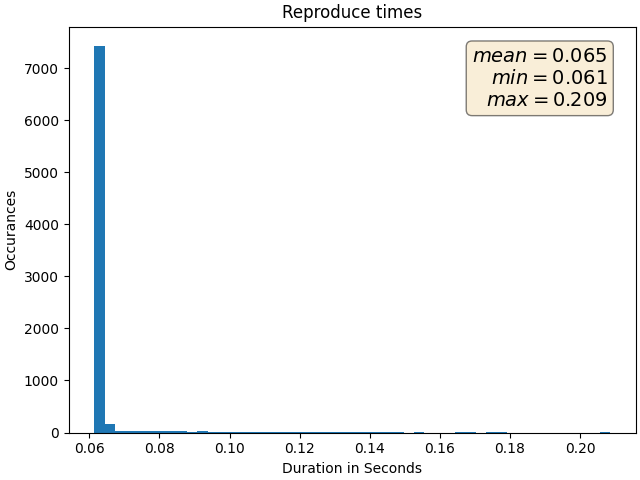
\includegraphics[width=0.8\textwidth]{Bilder/notebook_images/replay_times.png}
    \caption{Replay times on jetbot hardware}
    \label{fig:result_replay_times}
\end{figure} % a chart showing the replay times (max, min, mean)


\begin{figure}
    \centering
    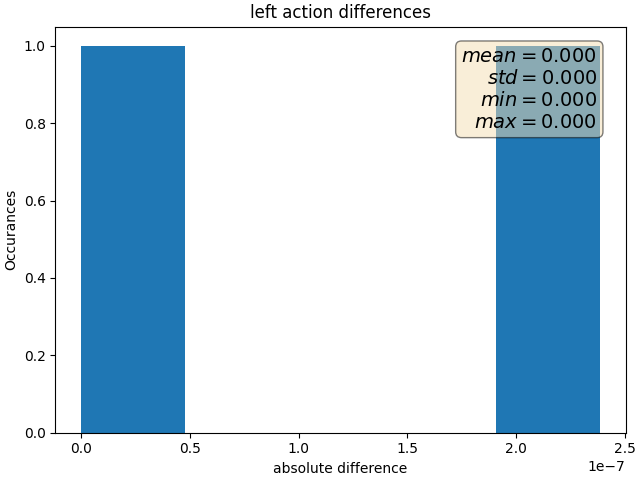
\includegraphics[width=0.45\textwidth]{Bilder/notebook_images/replay_outputs_action_left.png}
    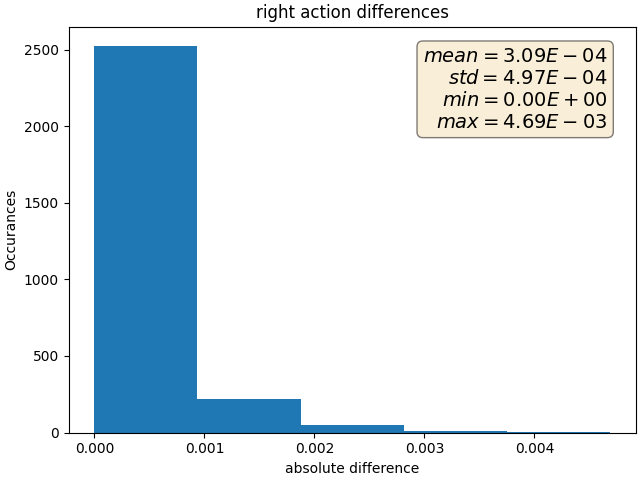
\includegraphics[width=0.45\textwidth]{Bilder/notebook_images/replay_outputs_action_right.png}
    \caption{Differences in policy outputs between recordings and replays on jetbot hardware}
    \label{fig:result_replay_outputs}
\end{figure} % a chart showing the replay outputs


\subsection{Experiment Results}

\paragraph{Replay times}

The replay times for the recordings on jetbot hardware are shown in figure \ref{fig:result_replay_times}. The maximum duration was $0.216$ seconds. The mean is much lower at $0.067$ seconds. The plot shows that the maximum duration was an extreme outlier.
Given the $fixedTimestepLength$ of $0.3$ seconds and the maximum duration of $0.216$ seconds, the hardware is fast enough to replay the episodes. This leaves at least $0.084$ seconds for the agent to recieve an image from the camera and send the new instruction to the motors.

The cameras used in the nvida jetbot are capable of capturing images with a resolution of $1280x720$ pixels at $60$ frames per second. This means the camera can capture an image every $0.0166$ seconds. The hardware is quick enough to compute actions in real time.

% times replay hardDistanceMixedLight: min 0.06319522857666016, mean 0.06662133265668013, max 0.21592259407043457

\paragraph{Policy Outputs}

The policy outputs from the recordings and the replays on jetbot hardware are nearly identical. The differences are shown in figure \ref{fig:result_replay_outputs}. The outputs were reproduced very closely. The maximum difference was $4.69e-03$.  This is difference is negligeable compared to the range of policy outputs $[-1,1]$.

% left action differences min [0.], max [0.00433731], mean 0.00030147546203806996, std 0.0004885991802439094
% right action differences min [0.], max [0.00468674], mean 0.00030857478850521147, std 0.000496754830237478

\subsection{Discussion}

The jetbot hardware is capable enough to compute the policy in real time. The differences of the policy outputs between the recordings and the replays are very small, the policy outputs were reproduced very closely. This suggests the differences in hardware and software do not impact the policy significantly.

\section{Other experiments}

\subsection{Sampling mode performance test}
\label{ref:sampling_mode_test_results}

The sampling mode performance test uses the Basic evaluation algorithm to evaluate an agent with derministic and non-deterministic sampling for each difficulty level. The success rates for the two sampling modes are compared to determine if the agent's performance is influenced by the sampling method. The sampling mode test was executed for all agents during the experimentation phase of this project using standard light.

\paragraph{Results}
The tests showed that the difference in performance for the sampling modes was very small for the trained policies. The results showed empirically that non-deterministic sampling leads to better success rates. Nevertheless some policies performed slightly worse using the non-deterministic sampling mode. The success rate was on average 1.7\% higher when using non-deterministic sampling. The biggest difference was 2.6\% for the medium difficulty setting \ref{fig:deterministic_check_result}.

\begin{figure}
    \centering
    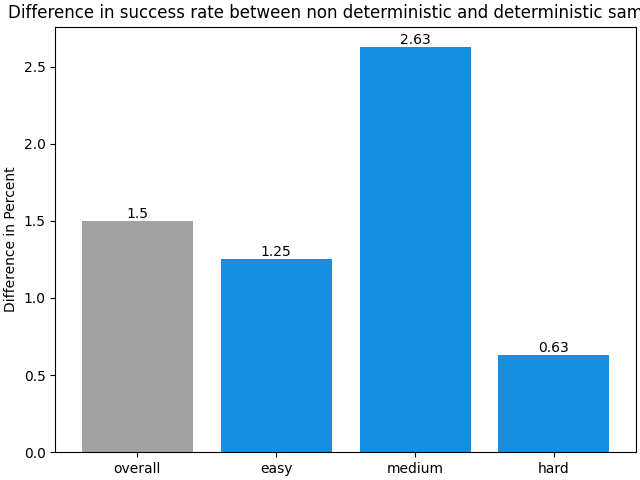
\includegraphics[width=0.8\textwidth]{Bilder/notebook_images/deterministic_check_results.png}
    \caption{Results of the deterministic check across all evaluations during the experimentation phase}
    \label{fig:deterministic_check_result}
\end{figure}

\paragraph{Discussion}
The test indicates that the non-deterministic sampling mode performes better, although the differences in performance are quite small. Given these results, the main evaluations for question 1 and 2 were conducted with non-deterministic sampling.

\subsection{Test identical start conditions}

% TODO run again

\subsection{Fresh obs improves}

fresh observation is slightly better than non-fresh observations
--> we can rerun the experiments for question 1 and 2 with fresh observations

rerun to see if the results are the same:

%|    fresh_better_by_easy_standard     | 0        |
%|    fresh_better_by_hard_standard     | -0.23    |
%|    fresh_better_by_medium_standard   | 0        |
%|    success_fresh_easy_standard       | 1        |
%|    success_fresh_hard_standard       | 0.76     |
%|    success_fresh_medium_standard     | 1        |
%|    success_nonfresh_easy_standard    | 1        |
%|    success_nonfresh_hard_standard    | 0.99     |
%|    success_nonfresh_medium_standard  | 1        |

% percall time 20 min vs 17 min
% 3    0.001    0.000 3704.876 1234.959 my_on_policy_algorithm.py:704(eval_model_track_wrapper_freshObs)
% 3    0.004    0.001 3077.651 1025.884 my_on_policy_algorithm.py:707(eval_model_track_wrapper_noFreshObs)

% retrain with freshObs?

\subsection{Jetbot generalization}

The policy was trained using the DifferentialJetBot shown in figure \ref{fig:jetbots}. The Jetbot Generalization test evaluates the same policy using the FourWheelJetBot. The policy is only evaluated on the standard light setting to save time.

\paragraph{Results}

\begin{figure}
    \centering
    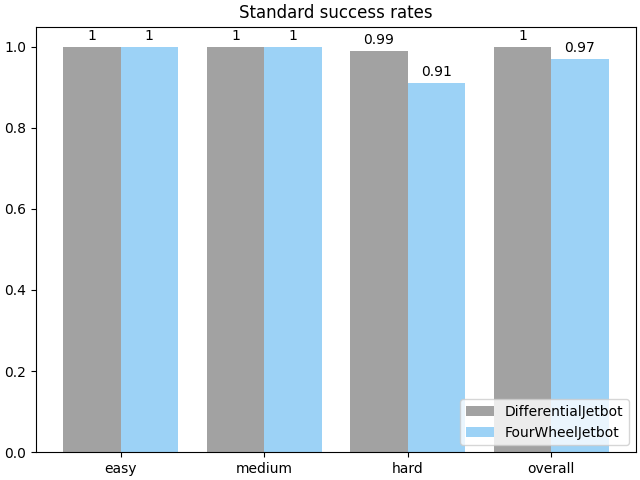
\includegraphics[width=0.45\textwidth]{Bilder/notebook_images/hardDistanceMixedLight_eval_jetbot_generalization_success_rates_barplot.png}
    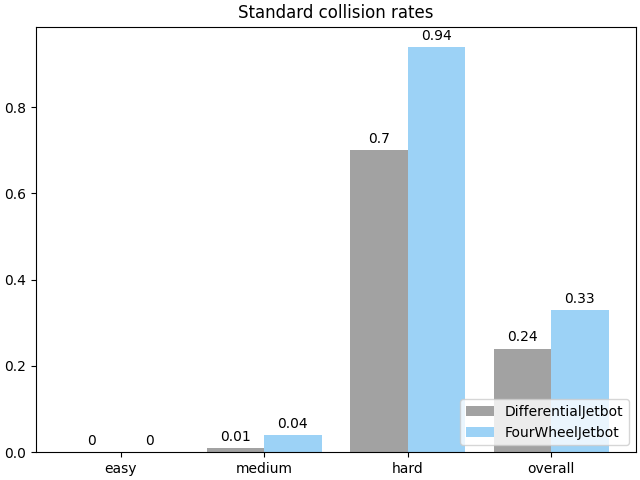
\includegraphics[width=0.45\textwidth]{Bilder/notebook_images/hardDistanceMixedLight_eval_jetbot_generalization_collision_rates_barplot.png}
    \caption{Evaluation of the DifferentialJetBot policy with both jetbot versions}
    \label{fig:result_jetbot_generalization}
\end{figure} % a chart showing the replay outputs

The policy evaluation achieves very high success rates for the FourWheelJetBot with 100\%, 100\% and 91\% for the easy, medium and hard tracks \ref{fig:result_jetbot_generalization}. The collision rates increase for higher difficulties with 0\%, 4\% and 94\%. 
The success and collision rates are slightly worse than on the DifferentialJetBot. The overall success rate of the FourWheelJetBot is 97\% compared to 100\% for the DifferentialJetBot. 

The overall collision rate is 33\% compared to 24\% for the DifferentialJetBot. Especially for the hard tracks the collision rate is much higher for the FourWheelJetBot with 94\% compared to 70\% for the DifferentialJetBot.
The collisions of the DifferentialJetBot were previously described as mainly being minor collisions where the agent scrapes the goal posts with its side. Analysis of the recorded videos shows that the collisions of the FourWheelJetBot are similar. However the agent scrapes the goals on its side for longer durations \ref{sec:fourwheel_collisions}.

% TODO explain why this longer collision is caused by the agent design?

% TODO record percentage of steps with collisions and compare?
% strong collisions here: hard_standard_FourWheelJetBot_env_0_video_2_topview

% TODO show and discuss failed episodes somewhere?

\paragraph{Discussion}

The policy that was trained on the DifferentialJetBot can be transfered to the FourWheelJetBot with only a slight decrease in performance.
The policy does not have to be retrained in this case. 


% TODO einheitliche Camel case für die jetbots verwenden (namen wie in Configs: DifferentialJetBot, FourWheelJetBot)